\section{Hardware}

\subsection{Motor und Controller}\label{subsec:MotorController}
Gemäss den Anforderungen an das Projekt, soll die gesamte Ansteuerung im Kleinspannungsbereich realisiert und mit Batterien versorgt werden. Diese liegt gemäss IEC 60449 Norm bei Gleichspannung $120V_{DC}$ und Wechselspannung $50V_{AC}$. Um einen Gleitschirmpiloten in die Luft zu heben, muss der Motor auch über ein grosses Drehmoment und genügend Leistung verfügen. Aus der Literatur Gleitsegelschlepp [Referenz 1](s.83) ist ersichtlich, dass der Gleitschirmpilot mit bis zu 10m/s gezogen wird. Aus den Richtlinien, welche der deutsche Gleitschirmverband erlassen hat, ist wiederrum ersichtlich, dass mit einer Zugkraft von bis zu 1kN bei Solopiloten und 1,3kN bei Tandempiloten gezogen werden darf [Referenz 2](Pkt. 24). Daraus lässt sich die maximale Leistung, welche das System auf den Gleitschirmpiloten ausüben darf ausrechnen [Referenz auf irgend ein Physikbuch]:


\begin{equation}
\centering
P_{Seil}=F \cdot \nu=1300N \cdot 10m/s=13kW
\label{eq:LeistungSeil}
\end{equation}

Da es sich um ein reales System handelt und deswegen im Motor, in Übertragung und Übersetzung Verluste auftreten, wird für die erste Handrechnung mit einem Gesamtwirkungsgrad des Systems von 80$\%$ gerechnet.

\begin{equation}
\centering
P_{Motor}==\frac{P_{Seil}}{\eta}=\frac{13kW}{0.8}=16.3kW
\label{eq:LeistungMotor}
\end{equation}

Da diese Leistung nicht über einen längeren Zeitraum geleistet werden muss, darf der Motor leicht unterdimensioniert werden. Als Realisierungsmöglichkeiten standen somit lediglich Wechselstrommotoren mit Wechselrichter, DC-Motoren oder Brushless DC (auch BLDC) Motoren in Frage kommen. Nachfolgend ist eine Auswahl an Motoren mit deren Controller aufgelistet.

\begin{figure}[H]
	\begin{center}
		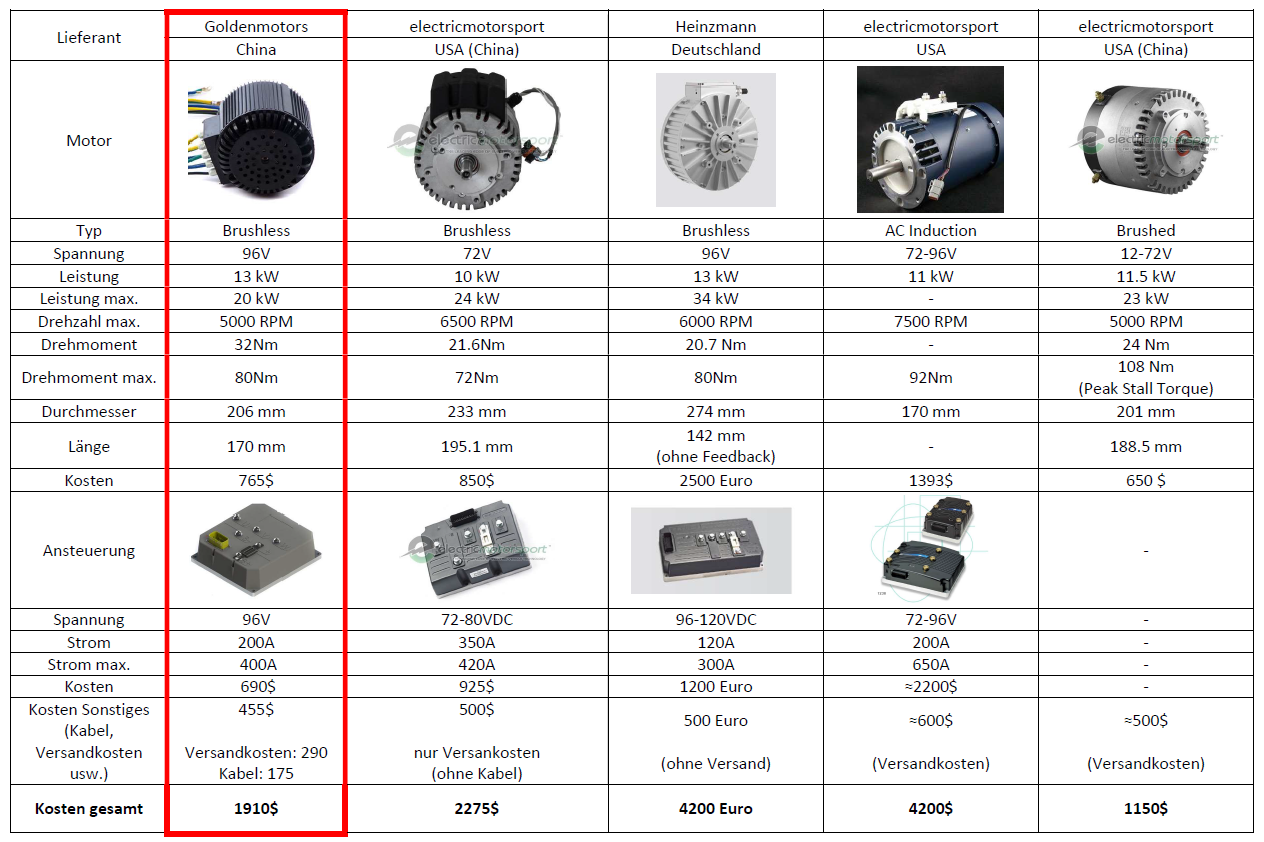
\includegraphics[width=160mm]{motor.png}
		\caption[Motorenvergleich]{Motor} %picture caption
		\label{fig:Funktion Dojo}
	\end{center}
\end{figure}

ES FOLGT TEXT ZU: WESHALB DIESER MOTOR AUSGEWÄHLT WURDE


Ausserdem wurde beim Motor die 96V Variante ausgewählt, da dieser durch die erhöhte Spannung einen kleineren Strom benötigt. Dadurch können kleinere Querschnitte gefahren werden, wodruch an Material eingespart werden kann.

\subsection{Energieversorgung}\label{subsec:Energieversorgung}

Damit die Einzugswinde betrieben werden kann, werden für die Energieversorgung Batterien verwendet. Wie im vorhergehenden Abschnitt \ref{subsec:MotorController} beschrieben, wurde ein Motor mit 96V Nennspannung ausgewählt. Aus diesem Grund ist es notwendig, Batterien mit derselben Versorgungsspannung zu verwenden. Durch die fortlaufende Weiterentwicklung von Akkumulatoren, stellte sich die Frage nach dem Typ und der notwendigen Kapazität für den Betrieb. Trotz der steilen Entwicklungskurve von Li-Ionen Akkus, sind sie im Vergleich zu kommerziellen Blei-Akkus, komplizierter und heikler in der Handhabung (Ladeschaltung mit Zellenüberwachung notwendig) und vor allem teurer. Es muss jedoch berücksichtigt werden, dass zyklenfeste Blei-Akkumulatoren teurer sind als herkömmliche Starterbatterien.
In nachfolgender Grafik werden einige Modelle dieser beiden Typen aufgelistet und verglichen. 
